\documentclass[14pt,a4paper]{extarticle}

\usepackage[left=3.5cm, right=1.5cm, top=2cm, bottom=2cm]{geometry}

\usepackage[utf8]{inputenc}
\usepackage[T2A]{fontenc}
\usepackage[english,russian]{babel}

\usepackage{amsmath}
\usepackage{amssymb}
\usepackage{bm}

\usepackage{graphicx}
\usepackage{float}
\usepackage{caption}
\usepackage{subcaption}
\renewcommand\thesubfigure{\asbuk{subfigure}}

\usepackage{enumitem}
\usepackage{siunitx}
\usepackage{cases}
\usepackage{dcolumn}

\usepackage{xcolor}
\usepackage{hyperref}
\usepackage{indentfirst}
\usepackage{hyphenat}

\linespread{1.3}
\setlength{\emergencystretch}{30pt}

\hyphenation{ма-те-ма-ти-ка вос-ста-нав-ли-вать}

\definecolor{linkcolor}{HTML}{0000D5}
\definecolor{urlcolor}{HTML}{0000D5}
\definecolor{citecolor}{HTML}{0000D5}

\hypersetup{
    pdfstartview=FitH,
    linkcolor=linkcolor,
    urlcolor=urlcolor,
    citecolor=citecolor,
    colorlinks=true
}

\bibliographystyle{IEEEtran}

\begin{document}


\thispagestyle{empty}

\begingroup
\fontsize{12}{14}\selectfont

\begin{center}
ПРАВИТЕЛЬСТВО РОССИЙСКОЙ ФЕДЕРАЦИИ

\vspace{0.2cm}

ФГАОУ ВО НАЦИОНАЛЬНЫЙ ИССЛЕДОВАТЕЛЬСКИЙ УНИВЕРСИТЕТ

\vspace{0.15cm}

«ВЫСШАЯ ШКОЛА ЭКОНОМИКИ»

\vspace{0.8cm}

Факультет компьютерных наук

\vspace{0.25cm}

Образовательная программа «Прикладная математика и информатика»

\vspace{1.45cm}

Отчет об исследовательском проекте на тему:

\vspace{0.35cm}

\textbf{Влияние типа данных на оптимизацию в физически информированных нейронных сетях}
\end{center}

\vspace{1.3cm}

\noindent
\begin{minipage}[t]{0.55\textwidth}
\raggedright
Выполнил:\\
студент группы БПМИ243\\
Тиханов Леонид Александрович
\end{minipage}


\vspace{1.1cm}

\noindent
\begin{minipage}[t]{0.55\textwidth}
\raggedright
Принял руководитель проекта:\\
Блуменау Марк Ильич \\
Преподаватель \\
Департамент больших данных и информационного поиска
\end{minipage}
\hfill
\begin{minipage}[t]{0.34\textwidth}
\centering
\end{minipage}

\vfill

\begin{center}
Москва 2026
\end{center}

\endgroup

\clearpage


\tableofcontents
\clearpage


\section*{Аннотация}
\addcontentsline{toc}{section}{Аннотация}

{Работа посвящена исследованию влияния численной точности на обучение физически информированных нейронных сетей. PINN - это нейронные сети, используемые для решения дифференциальных уравнений. В большом количестве работ описаны проблемы с их обучением, так называемые failure modes. Вопрос работы состоит в том, как переход от FP32 к FP64 влияет на оптимизацию PINN. }

Эксперименты на классических дифференциальных уравнениях показали, что для задач со сложным ландшафтом потерь переход к формату FP64 позволяет преодолеть оптимизационные барьеры. Но в случае простых задач или наоборот сложных нелинейных систем повышение разрядности не является универсальным решением

\clearpage

\section{Введение}

В этой работе PINN используются как модель для сравнения численной точности при обучении. Основная цель - проверить, как одинаковая архитектура ведёт себя при вычислениях в FP32 и FP64.

На практике зачастую во время обучения PINN возникают нестабильности. Возможна ситуация, когда функция потерь принимает достаточно небольшие значения, а реальная ошибка относительно точного решения остается существенной. В литературе это принято называть failure modes. 

В рамках этой проблемы особого внимания требует численная точность вычислений. Как правило, в глубинном обучении используется FP32 или более низкие форматы для ускорения обучения. При этом ошибки округления могут влиять не только на финальный результат, но и на процесс сходимости.

Целью работы является исследование влияния FP32 и FP64 на качество и устойчивость обучения физически информированных нейронных сетей.


\section{Обзор литературы}

\subsection{Physics-Informed Neural Networks}

Физически информированные нейронные сети появились как способ объединить нейросетевую аппроксимацию и информацию о физической модели задачи. Базовая идея подхода была сформулирована в работе Raissi, Perdikaris и Karniadakis~\cite{raissi2019physics}. В отличие от обычного обучения по данным, PINN использует не только значения функции в известных точках, но и дифференциальное уравнение, которому должно удовлетворять искомое решение.

В прямой задаче требуется найти функцию $u(x,t)$, удовлетворяющую некоторому дифференциальному уравнению
\[
    \mathcal{N}[u](x,t)=0
\]
где $\mathcal{N}$ -  дифференциальный оператор. В PINN решение заменяется нейросетевой аппроксимацией $u_\theta(x,t)$. После этого производные, входящие в уравнение, вычисляются с помощью автоматического дифференцирования. Таким образом модель одновременно приближает решение на известных данных и пытается удовлетворять свойствам точного решения, описанным с помощью уравнения.

Как правило функция потерь PINN выглядит как
\[
    \mathcal{L}
    =
    \mathcal{L}_{data}
    +
    \lambda_f \mathcal{L}_{f}
    +
    \lambda_{bc}\mathcal{L}_{bc}
    +
    \lambda_{ic}\mathcal{L}_{ic}.
\]
$\mathcal{L}_{data}$ отвечает за ошибку на известных наблюдениях, $\mathcal{L}_{f}$~--- за невязку дифференциального уравнения во внутренних точках области, $\mathcal{L}_{bc}$ и $\mathcal{L}_{ic}$ задают выполнение граничных и начальных условий. Если данных мало, физическая часть loss позволяет всё равно ограничить множество возможных решений и использовать известную структуру задачи.

В работе~\cite{raissi2019physics} выделяют две постановки задачи: прямая и обратная. В случае прямой задачи известны параметры уравнения и необходимо искать решение. В обратной задаче параметры уравнения не известны и необходимо восстанавливать их по наблюдениям. В данной работе рассматривается прямая задача. 

Так же в PINN различают непрерывные и дискретные по времени подходы~\cite{raissi2019physics}. В непрерывном варианте сеть аппроксимирует решение на всей области, а производные по времени и пространству считаются напрямую через автоматическое дифференцирование. В дискретном варианте используются временные методы, например схемы Рунге--Кутты, связывающие значения решения на соседних временных слоях. В данной работе используется непрерывная постановка.

Главное преимущество PINN состоит в том, что мы используем известную нам информацию о физической модели в виде уравнения. Это делает метод привлекательным для задач научного машинного обучения, где известна модель процесса, но получение большого количества точных данных может быть дорогим или невозможным.

\subsection{Failure modes при обучении PINN}

Несмотря на простую идею, PINN часто оказываются сложными в оптимизации. На практике возможна ситуация, когда значение функции потерь становится малым, но реальная ошибка относительно точного решения остаётся большой. Такие ситуации принято называть failure modes.

Одна из ключевых работ по этой теме - Characterizing possible failure modes in physics-informed neural networks~\cite{krishnapriyan2021characterizing}. В ней авторы показывают, что failure modes могут возникать не из-за недостаточной выразительности сети, а из-за сложности оптимизации. Авторы связывают это с ландшафтом функции потерь и показывают, что разные варианты обучения могут существенно менять результат.


\subsection{Сэмплирование точек и распространение ошибки}

Альтернативным подходом к решению проблемы failure modes является адаптивное сэмплирование. В классическом варианте эти точки выбираются случайно по всей области. Но в какой-то момент может образоваться ситуация, что модель лучше выучила какие-то определенные области (скорее всего более простые) и хуже другие.

 Например, в стратегии R3 Sampling~\cite{daw2022r3} набор коллокационных точек динамически обновляется: алгоритм сохраняет точки с высокой невязкой и удаляет те, где сеть уже хорошо аппроксимировала решение. Успешность таких методов на классических бенчмарках доказывает, что стагнация оптимизатора может быть вызвана не только вычислительной точностью, но и неравномерным распределением градиентов по пространственной области.

\subsection{Оптимизация и ландшафт функции потерь}

Проблемы PINN также активно рассматриваются с точки зрения ландшафта функции потерь и выбора оптимизатора. В работе Challenges in Training PINNs: A Loss Landscape Perspective авторы связывают трудности обучения с плохой обусловленностью loss и показывают, что стандартные методы оптимизации могут быть недостаточными~\cite{rathore2024challenges}.

Как правило при обучении PINN сначала используют Adam для получения хорошего начального приближения, а затем спомощью L-BFGS уточняют решение.  В работе~\cite{rathore2024challenges} подчёркивается, что Adam и L-BFGS по отдельности могут работать хуже, чем их последовательное применение. При этом даже связка Adam+L-BFGS не всегда полностью решает проблему плохой обусловленности. Авторы предлагают более сложный метод NysNewton-CG, который использует приближение второго порядка и может давать улучшение на ряде задач.

Данные статьи объясняют то, почему в экспериментах разумнее использовать Adam+L-BFGS вместе а не по отдельности. Следовательно, для корректного сравнения типов данных необходимо фиксировать архитектуру и метод оптимизации

\subsection{Низкая точность в классическом deep learning}

В классическом глубинном обучении существует тренд на то, что развитие вычислений связано со снижением размерности данных. Стандартным форматом данных можно считать FP32, но часто для ускорения обучения и уменьшения расхода памяти применяются более компактные форматы. Это объясняется тем, что многие нейросетевые модели при использовании специальных методов стабилизации обучения устойчивы к небольшим ошибкам округления.

Одна из ранних работ в этом направлении - Deep Learning with Limited Numerical Precision~\cite{gupta2015limited}. В ней показывается, что при использовании стохастического округления обучение нейросетей возможно даже при заметно ограниченной численной точности. Такой подход позволяет уменьшить вычислительные затраты по сравнению с FP32 и при этом сохранить приемлемое качество в ряде задач.

Стоит упомянуть так же и квантование нейронных сетей. Обзор A Survey of Quantization Methods for Efficient Neural Network Inference систематизирует методы перевода весов и активаций из высокоточных форматов в более компактные представления~\cite{gholami2021survey}. Главная цель таких методов - ускорить инференс и уменьшить потребление памяти. Зачастую это полезно в задачах компьютерного зрения, обработки языка и рекомендательных систем.

При этом стоит понимать, что в случае PINN ситуация иная. В отличии от классических задач в PINN дополнительно вычисляются производные и невязки физических уравнений, которые могут быть достаточно чувствительны к ошибкам округления.


\subsection{Смешанная точность в scientific machine learning}

В работе Speeding up and reducing memory usage for scientific machine learning via mixed precision исследуется использование смешанной точности в задачах SciML~\cite{hayford2024mixed}. В ней показывают, что комбинация разных численных форматов может уменьшить расход памяти и ускорить вычисления. Однако для PINN низкая точность требует осторожности, поскольку при обучении вычисляются производные и невязки уравнения.

\subsection{FP64 как возможное объяснение failure modes}

Исходя из прошлых идей, можно прийти к идее увеличения точности представления данных. Это сделали авторы статьи FP64 is All You Need: Rethinking Failure Modes in Physics-Informed Neural Networks~\cite{wang2025fp64}. Авторы оспаривают устоявшееся объяснение проблемы обучения PINN через локальные минимумы функции потерь. Они утверждают, что при переходе от FP32 к FP64 оптимизация в ряде задач продолжает снижать ошибку там, где FP32 фактически останавливается. Эта идея используется в моей работе как основная мотивация, но проверяется на другом наборе задач.

В статьях, исследующих влияние точности на обучение PINN, обычно выделяют две главные гипотезы о том, как именно ведет себя модель в процессе оптимизации. Это Same-Basin гипотеза  и Loss-Barrier гипотеза.
В первом случае мы считаем, что независимо от того, учим мы модель в FP32 или в FP64, она попадает в одну и ту же область локального минимума на ландшафте функции потерь. Разница лишь в том, что меньшему типу данных банально не хватает точности дробной части, чтобы ландшафт дна для него был ощутим. Из-за вычислительного шума при подсчете градиентов модель просто останавливается чуть выше минимума. Формат FP64 в этом случае просто позволяет аккуратно спуститься в этой же яме до самого конца.
Loss-Barrier гипотеза же предполагает, что ландшафт ошибки очень сложный и содержит преграды. При обучении в FP32 модель быстро упирается в такую преграду - градиенты становятся слишком маленькими, оптимизатор перестает их "видеть" и застревает в плохом решении. Переход на FP64 дает оптимизатору достаточное разрешение, чтобы преодолеть эти барьеры и выйти из области локального минимума.


Эта работа опирается на идею статьи про роль FP64 в PINN, но проверяет её на другом наборе задач: Heat1D, Helmholtz1D, Convection1D и Burgers1D.



\section{Постановка задачи}

Цель работы - оценить влияние перехода от формата FP32 к FP64 на процесс оптимизации PINN вряде одномерных задач.

\subsection{Общая схема PINN}

В прямой задаче необходимо найти решение $u(x,t)$ некоторого дифференциального уравнения. В PINN мы полчаем аппроксимацию решения
\[
    u_\theta(x,t)
\]

Дифференциальное уравнение можно записать в общем виде:
\begin{equation}
    \mathcal{N}[u](x,t) = 0
    \label{eq:general_pde}
\end{equation}
где $\mathcal{N}$ - дифференциальный оператор. Подставляя решение нейросети $u_\theta$ получается невязка PDE:
\begin{equation}
    PDE_\theta(x,t) = \mathcal{N}[u_\theta](x,t)
    \label{eq:pde_residual}
\end{equation}

\subsection{Функция потерь}

PINN обучается минимизацией следующей функции потерь:
\begin{equation}
    \mathcal{L}
    =
    \lambda_{pde}\mathcal{L}_{pde}
    +
    \lambda_{ic}\mathcal{L}_{ic}
    +
    \lambda_{bc}\mathcal{L}_{bc}.
    \label{eq:pinn_loss}
\end{equation}

$\mathcal{L}_{pde}$ отвечает за невязку дифференциального уравнения, $\mathcal{L}_{ic}$ задаёт ошибку на начальных точках, а $\mathcal{L}_{bc}$ задает ошибку на граничных точках.

Физическая часть функции потерь считается по набору коллокационных точек:
\begin{equation}
    \mathcal{L}_{pde}
    =
    \frac{1}{N_pde}
    \sum_{i=1}^{N_pde}
    PDE_\theta(x_i,t_i)^2
    \label{eq:pde_loss}
\end{equation}
где $N_f$ - число внутренних точек, в которых вычисляется невязка уравнения

Ошибки на начальных и граничных условиях считаются как среднеквадратичные ошибки между предсказанием сети и известными значениями:
\begin{equation}
    \mathcal{L}_{ic}
    =
    \frac{1}{N_{ic}}
    \sum_{i=1}^{N_{ic}}
    \left(
        u_\theta(x_i,0) - u_0(x_i)
    \right)^2,
    \label{eq:ic_loss}
\end{equation}
\begin{equation}
    \mathcal{L}_{bc}
    =
    \frac{1}{N_{bc}}
    \sum_{i=1}^{N_{bc}}
    \left(
        u_\theta(x_i,t_i) - u_{bc}(x_i,t_i)
    \right)^2
    \label{eq:bc_loss}
\end{equation}


\subsection{Рассматриваемые PDE}

В экспериментах используются одномерные дифференциальные уравнения, которые отличаются по сложности обучения. Формулы рассматриваемых задач приведены в таблице~\ref{tab:pde_equations}.

\begin{table}[H]
\centering
\caption{Рассматриваемые уравнения}
\label{tab:pde_equations}
\begin{tabular}{lll}
\hline
Задача & Уравнение & Параметр \\
\hline
Heat1D &
$u_t = \alpha u_{xx}$ &
$\alpha$ \\

Helmholtz1D &
$u_{xx} + (m\pi)^2 u = f(x)$ &
$m$ \\

Convection1D &
$u_t + \beta u_x = 0$ &
$\beta$ \\

Burgers1D &
$u_t + u u_x = \nu u_{xx}$ &
$\nu$ \\
\hline
\end{tabular}
\end{table}

Уравнение Heat1D используется в качестве базовой проверки, поскольку оно не обладает выраженными градиентными барьерами.

В задаче Helmholtz1D рассматриваются разные значения параметра $m$. Увеличение m увеличивает частоту решения и усложняет задачу.

Задача Convection1D рассматривается как дополнительный эксперимент, близкий к экспериментам из статьи~\cite{wang2025fp64}.

 Для задачи Burgers1D FP64 не всегда даёт устойчивое преимущество над FP32.

\subsection{Сравниваемые типы данных}

В работе сравниваются два формата вычислений: FP32 и FP64. Для честного сравнения в выбранный тип данных переводятся параметры модели, входные точки и вычисления функции потерь. 

Основной интерес представляет сравнение FP32 и FP64. В PINN обучение зависит от вычисления производных и малых значений физической невязки. Поэтому ошибки округления могут влиять не только на финальную точность, но и на сам процесс оптимизации.


\subsection{Метрики качества}

Для оценки качества решений используются следующие метрики:
Среднеквадратичная ошибка:
\begin{equation}
    MSE =
        \frac{1}{N}
        \sum_{i=1}^{N}
        (u_i - \hat{u}_i)^2
    \label{eq:rmse}
\end{equation}

Относительная L2-ошибка:
\begin{equation}
    relative\ L2 =
    \frac{
        \|u - \hat{u}\|_2
    }{
        \|u\|_2
    }
    \label{eq:relative_l2}
\end{equation}

$u$ обозначает точное решение на тестовой сетке, а $\hat{u}$ - предсказание нейронной сети. Финальное сравнение проводится по лучшей L2-ошибке.




\section{Реализация экспериментов}

\subsection{Архитектура нейронной сети}

В качестве модели используется полносвязная нейронная сеть. Для нестационарных задач Heat1D, Burgers1D и Convection1D входом сети является пара координат $(x,t)$. Для стационарной задачи Helmholtz1D входом является только пространственная координата $x$.

Фактический размер модели зависит от конкретного экспериментального блока. В основных запусках использовались следующие конфигурации.

\begin{table}[H]
\centering
\caption{Основные параметры архитектуры}
\label{tab:model_params_real}
\begin{tabular}{llll}
\hline
Задача & Размер скрытого слоя & Число слоёв \\
\hline
Helmholtz1D & 128 & 4 \\
Convection1D, $\beta=30$ & 256 & 3 \\
Burgers1D & 256 & 4 \\
\hline
\end{tabular}
\end{table}

\subsection{Автоматическое дифференцирование и вычисление невязок}
Производные в вычислении невязки дифференциального уравнения считаются через
 \texttt{torch.autograd.grad}.

Heat1D уравнение
\[
    u_t = \alpha u_{xx}
\]
Поэтому невязка имеет вид:
\[
    PDE_\theta(x,t)
    =
    \frac{\partial u_\theta}{\partial t}
    -
    \alpha
    \frac{\partial^2 u_\theta}{\partial x^2}
\]
Точное решение для этой задачи задаётся формулой
\[
    u(x,t)=\exp(-\pi^2 \alpha t)\sin(\pi x)
\]

Burgers1D уравнение
\[
    u_t + u u_x = \nu u_{xx}
\]
Невязка имеет следующий вид
\[
    PDE_\theta(x,t)
    =
    \frac{\partial u_\theta}{\partial t}
    +
    u_\theta
    \frac{\partial u_\theta}{\partial x}
    -
    \nu
    \frac{\partial^2 u_\theta}{\partial x^2}
\]
Начальное условие
\[
    u(x,0)=-\sin(\pi x)
\]
На границах $x=-1$ и $x=1$ используется нулевое условие.

Convection1D уравнение
\[
    u_t + \beta u_x = 0
\]
Соответствующая невязка
\[
    PDE_\theta(x,t)
    =
    \frac{\partial u_\theta}{\partial t}
    +
    \beta
    \frac{\partial u_\theta}{\partial x}
\]
Точное решение
\[
    u(x,t)=\sin(x-\beta t)
\]
Для этой задачи область по $x$ задаётся на отрезке $[0,2\pi]$, а по времени на отрезке $[0,1]$

Для Helmholtz1D используется стационарная задача. Точное решение задано как
\[
    u(x)=\sin(m\pi x).
\]
Правая часть строится в виде
\[
    f(x) =
    \left(\lambda - (m\pi)^2\right)\sin(m\pi x).
\]
Невязка уравнения
\[
    u_{xx} + \lambda u = f(x)
\]
Дополнительно используется нормировка невязки на величину
\[
    |\lambda - (m\pi)^2|
\]
Нормировка нужна, чтобы задача Helmholtz при разных $m$ измерялась в одном масштабе. Иначе при увеличении $m$ правая часть уравнения становится больше, а вместе с ней искусственно растёт и PDE-loss.
То есть фактически невязка для Helmholtz1D имеет вид
\[
    PDE_\theta(x)
    =
    \frac{
        u_{\theta,xx}(x)
        +
        \lambda u_\theta(x)
        -
        f(x)
    }{
        |\lambda - (m\pi)^2|
    }.
\]

Физическая часть функции потерь во всех задачах считается как средний квадрат невязки:
\[
    \mathcal{L}_{pde}
    =
    \frac{1}{N_f}
    \sum_{i=1}^{N_f}
    PDE_\theta(x_i,t_i)^2
\]

\subsection{Оптимизация: Adam + L-BFGS}

Обучение проводится в два этапа
\[
    Adam + L\text{-}BFGS
\]
Сначала используется Adam, который помогает получить начальное приближение.

В основных отчётных запусках использовались разные режимы обучения для разных PDE.

\begin{table}[H]
\centering
\caption{Основные параметры обучения экспериментах}
\label{tab:train_params_real}
\begin{tabular}{lllll}
\hline
Задача & $N_f$ & $N_{ic}$ & $N_{bc}$ & Оптимизация \\
\hline
Helmholtz1D & 5000 & 0 & 2 & Adam 10000 + L-BFGS 1000/2000 \\
Convection1D, $\beta=30$ & 4225 & 65 & 65 & L-BFGS 4000 \\
Burgers1D & 10000 & 800 & 800 & Adam 3000 + L-BFGS 2000 \\
\hline
\end{tabular}
\end{table}

В Helmholtz1D начальное условие отсутствует, так как задача стационарная. Для неё используются внутренние точки на $x\in[0,1]$ и граничные точки $x=0$ и $x=1$. В основных Helmholtz-запусках также использовалось периодическое обновление коллокационных точек.



\section{Результаты экспериментов}

В этом разделе приведены результаты сравнения FP32 и FP64.

\begin{figure}[H]
    \centering
    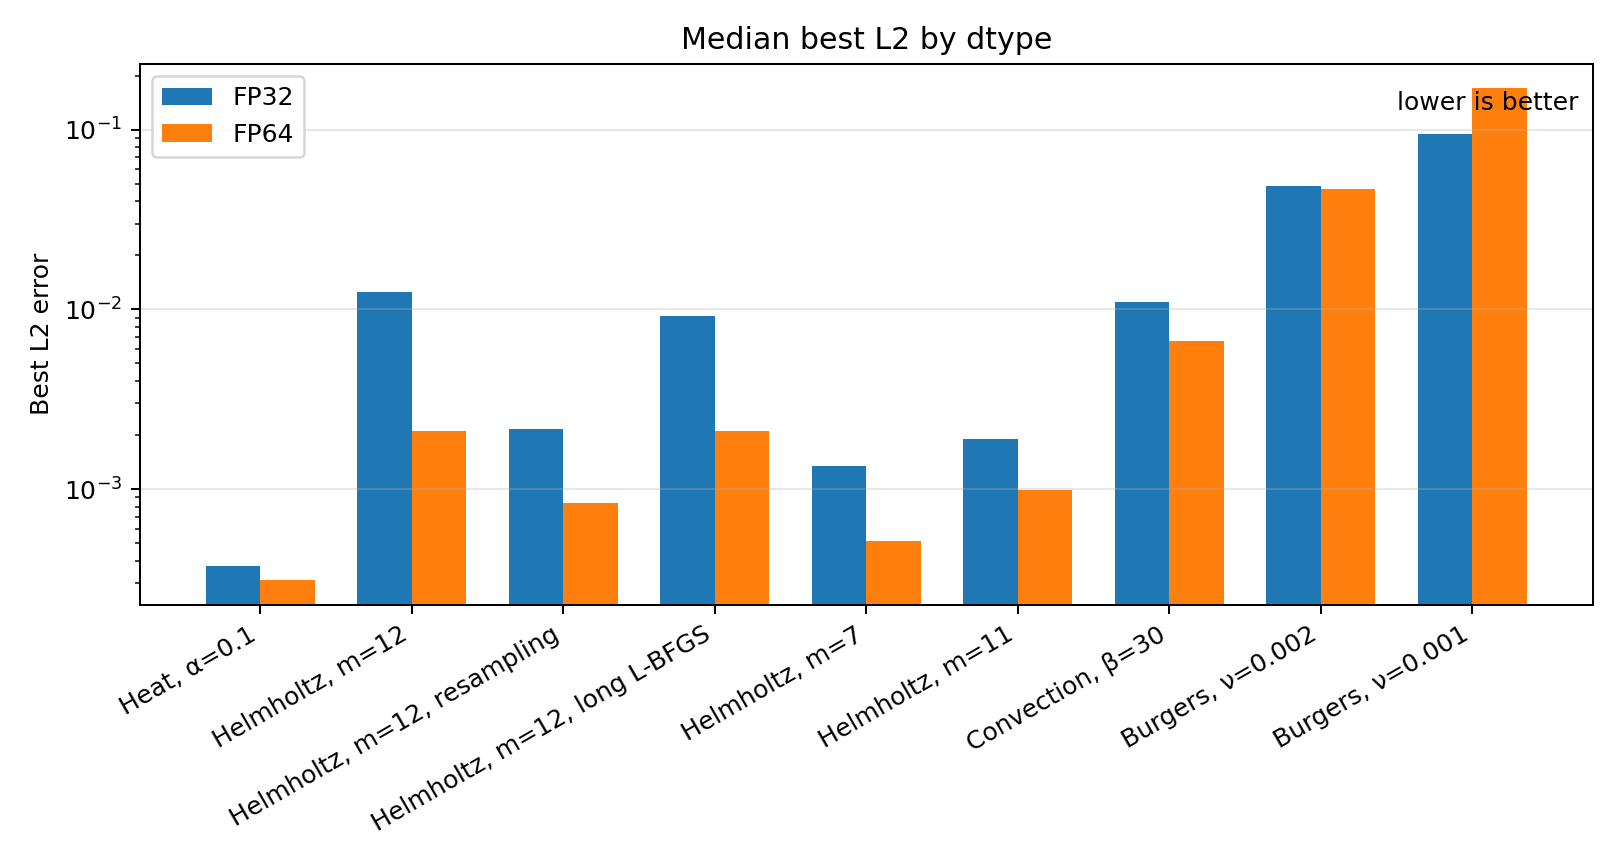
\includegraphics[width=0.9\textwidth]{report_results/figures/report_main_best_l2_by_dtype.png}
    \caption{Сравнение медианной лучшей относительной L2-ошибки для основных запусков}
    \label{fig:main_best_l2}
\end{figure}

На рисунке~\ref{fig:main_best_l2} видно, что поведение разных задач заметно отличается. Heat1d достаточно простая задача и в обоих случаях ошибка доволно маленькая, на уравне погрешности от случайности. Для Helmholtz1D FP64 дает значительное улучшение. В случае Convection1D Fp64 оказывается немного лучше. А для Burgers1D использование FP64 не дало выигрыша в качестве.

\begin{figure}[H]
    \centering
    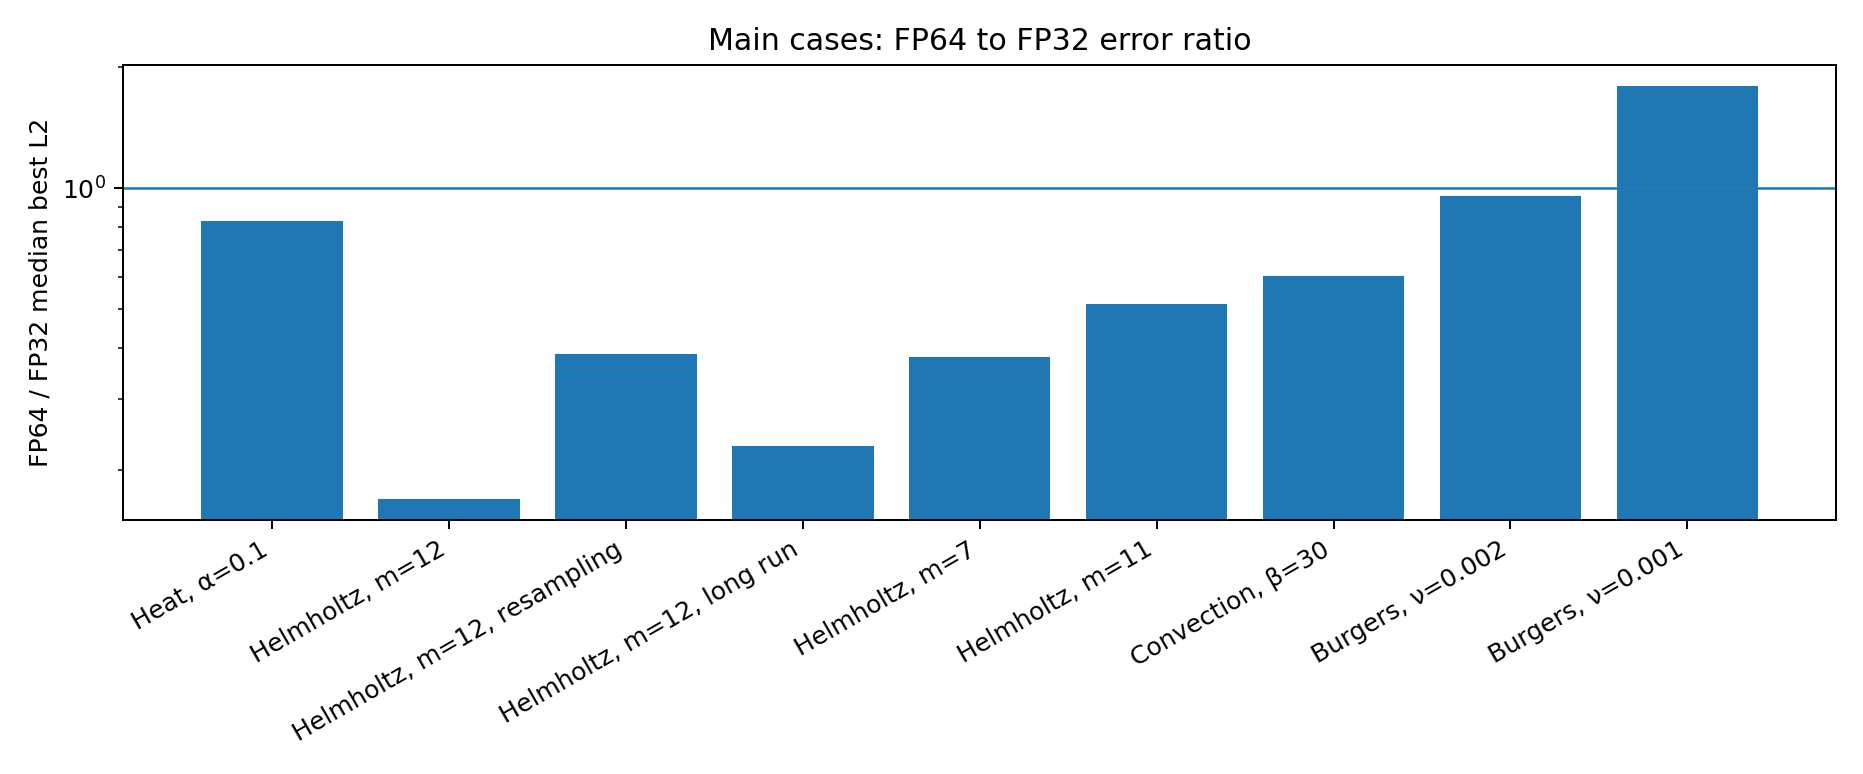
\includegraphics[width=0.9\textwidth]{report_results/figures/report_main_fp64_fp32_ratio.png}
    \caption{Отношение медианной ошибки FP64 к медианной ошибке FP32}
    \label{fig:main_ratio}
\end{figure}

На рисунке~\ref{fig:main_ratio} значение меньше единицы означает, что FP64 дал меньшую ошибку, чем FP32. Можно сравнить относительное отличие FP32 и FP64. Становится ясно, что наибольшая разница 

\subsection{Heat1D}

Это сравнительно простая задача, поэтому от неё не ожидается failure mode поведения.

\begin{table}[H]
\centering
\caption{Результаты на Heat1D}
\label{tab:heat_results}
\begin{tabular}{lllll}
\hline
Задача & Параметр & Seed FP32/FP64 & FP32 best L2 & FP64 best L2 \\
\hline
Heat1D & $\alpha=0.1$ & 3/3 & \num{3.753e-4} & \num{3.107e-4} \\
\hline
\end{tabular}
\end{table}

В таблице~\ref{tab:heat_results} видно, что ожидаемо обе точности дают достаточно малую схожую ошибку. Это означает, что обе точности работают достаточно хорошо на такой простой задаче и никаких проблем с обучением не возникает. 

\subsection{Helmholtz1D}

В задаче Helmholtz1D при увеличении `m` увеличивается частота точного решения и его приближение становится 

\begin{table}[H]
\centering
\caption{Основные результаты на Helmholtz1D}
\label{tab:helmholtz_results}
\begin{tabular}{lllll}
\hline
Кейс & Seed FP32/FP64 & FP32 best L2 & FP64 best L2 & FP64/FP32 \\
\hline
$m=12$ & 2/2 & \num{1.253e-2} & \num{2.114e-3} & \num{0.169} \\
$m=12$, resampling & 2/2 & \num{2.160e-3} & \num{8.340e-4} & \num{0.386} \\
$m=12$, long run & 2/2 & \num{9.213e-3} & \num{2.114e-3} & \num{0.229} \\
$m=7$, resampling & 2/2 & \num{1.348e-3} & \num{5.144e-4} & \num{0.382} \\
$m=11$, resampling & 2/2 & \num{1.906e-3} & \num{9.833e-4} & \num{0.516} \\
\hline
\end{tabular}
\end{table}

Во всех строках таблицы~\ref{tab:helmholtz_results} медианная ошибка FP64 ниже медианной ошибки FP32. Наиболее сильный эффект виден в запуске $m=12$ медианная лучшая относительная L2-ошибка уменьшается с $\num{1.253e-2}$ для FP32 до $\num{2.114e-3}$ для FP64. Отношение FP64/FP32 равно $\num{0.169}$, то есть ошибка FP64 составляет примерно 17\% от ошибки FP32.

Для другого запуска с $m=12$ и ресемплированием FP64 также лучше: ошибка уменьшается с $\num{2.160e-3}$ до $\num{8.340e-4}$. Для $m=7$ и $m=11$ преимущество FP64 тоже сохраняется, хотя величина выигрыша отличается.

\begin{figure}[H]
    \centering
    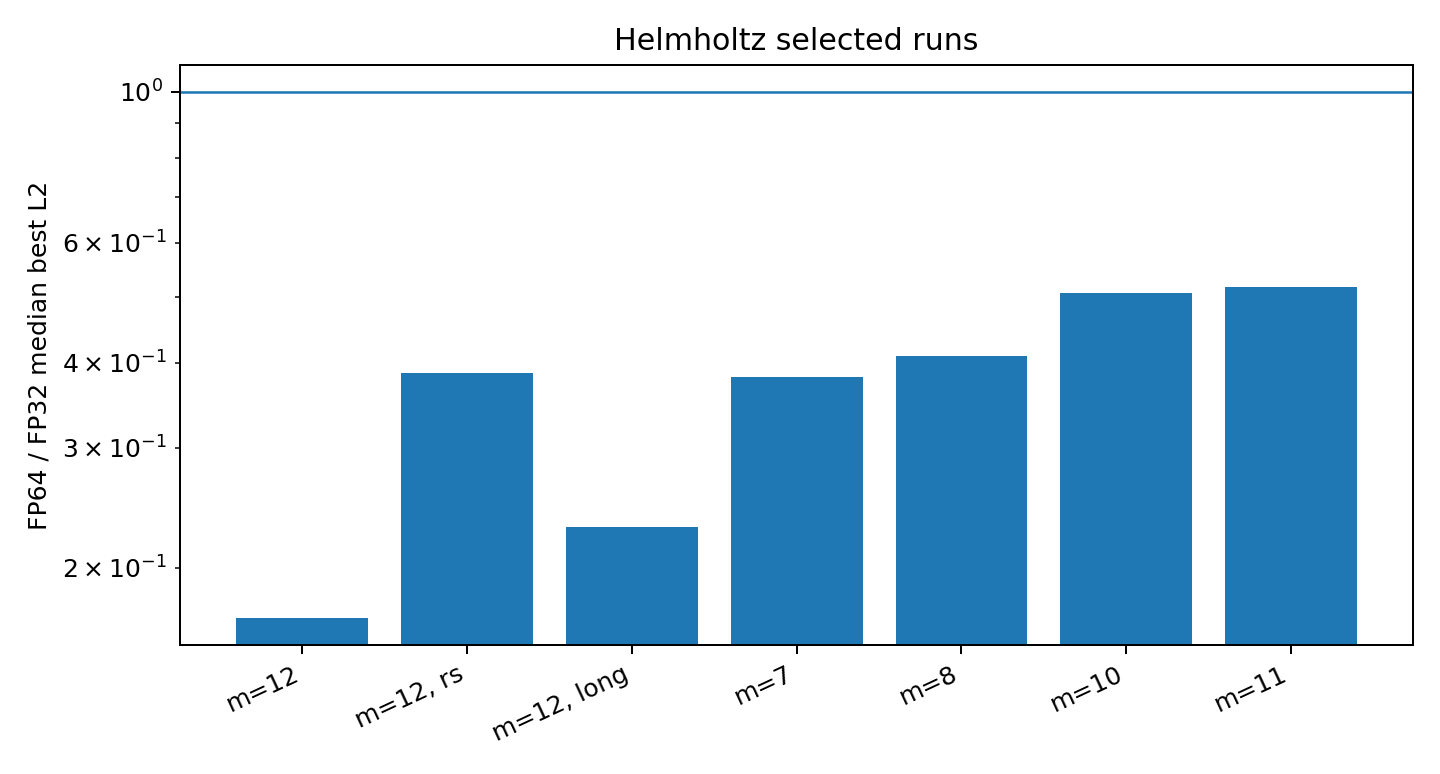
\includegraphics[width=0.9\textwidth]{report_results/figures/report_helmholtz_main_ratio.png}
    \caption{Отношение ошибки FP64 к ошибке FP32 для Helmholtz1D}
    \label{fig:helmholtz_ratio}
\end{figure}

Рисунок~\ref{fig:helmholtz_ratio} показывает, что для основных Helmholtz-запусков отношение FP64/FP32 находится ниже единицы. Это означает, что повышенная точность в этих случаях действительно помогает оптимизации прийти к более точному решению.

\begin{figure}[H]
    \centering
    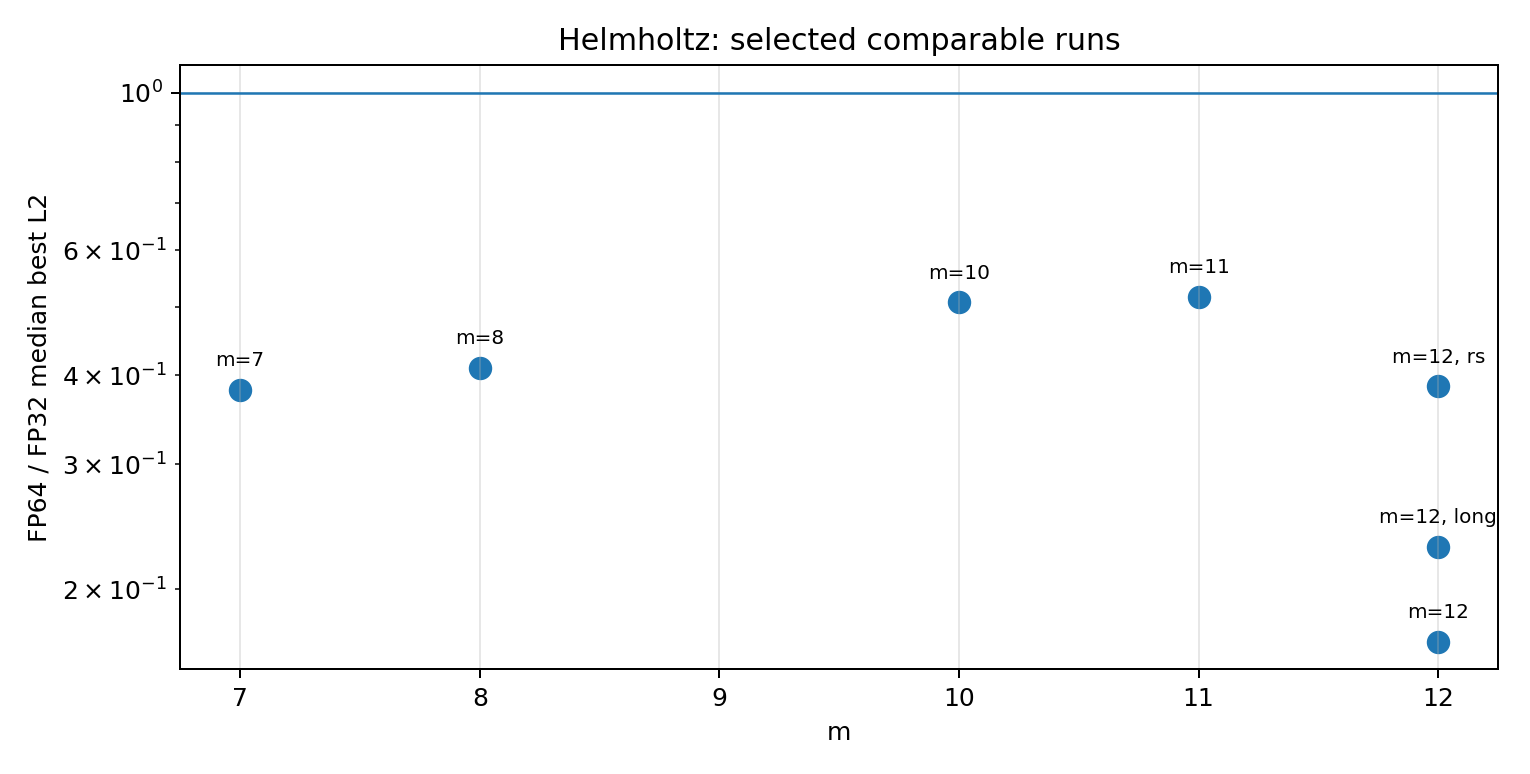
\includegraphics[width=0.9\textwidth]{report_results/figures/report_helmholtz_rs_sweep.png}
    \caption{Сравнение Helmholtz1D для разных значений параметра $m$}
    \label{fig:helmholtz_sweep}
\end{figure}

На рисунке~\ref{fig:helmholtz_sweep} видно, что преимущество FP64 проявляется не только для одного значения $m$.

Отдельно рассмотрим кривые обучения для основного случая $m=12$.

\begin{figure}[H]
    \centering
    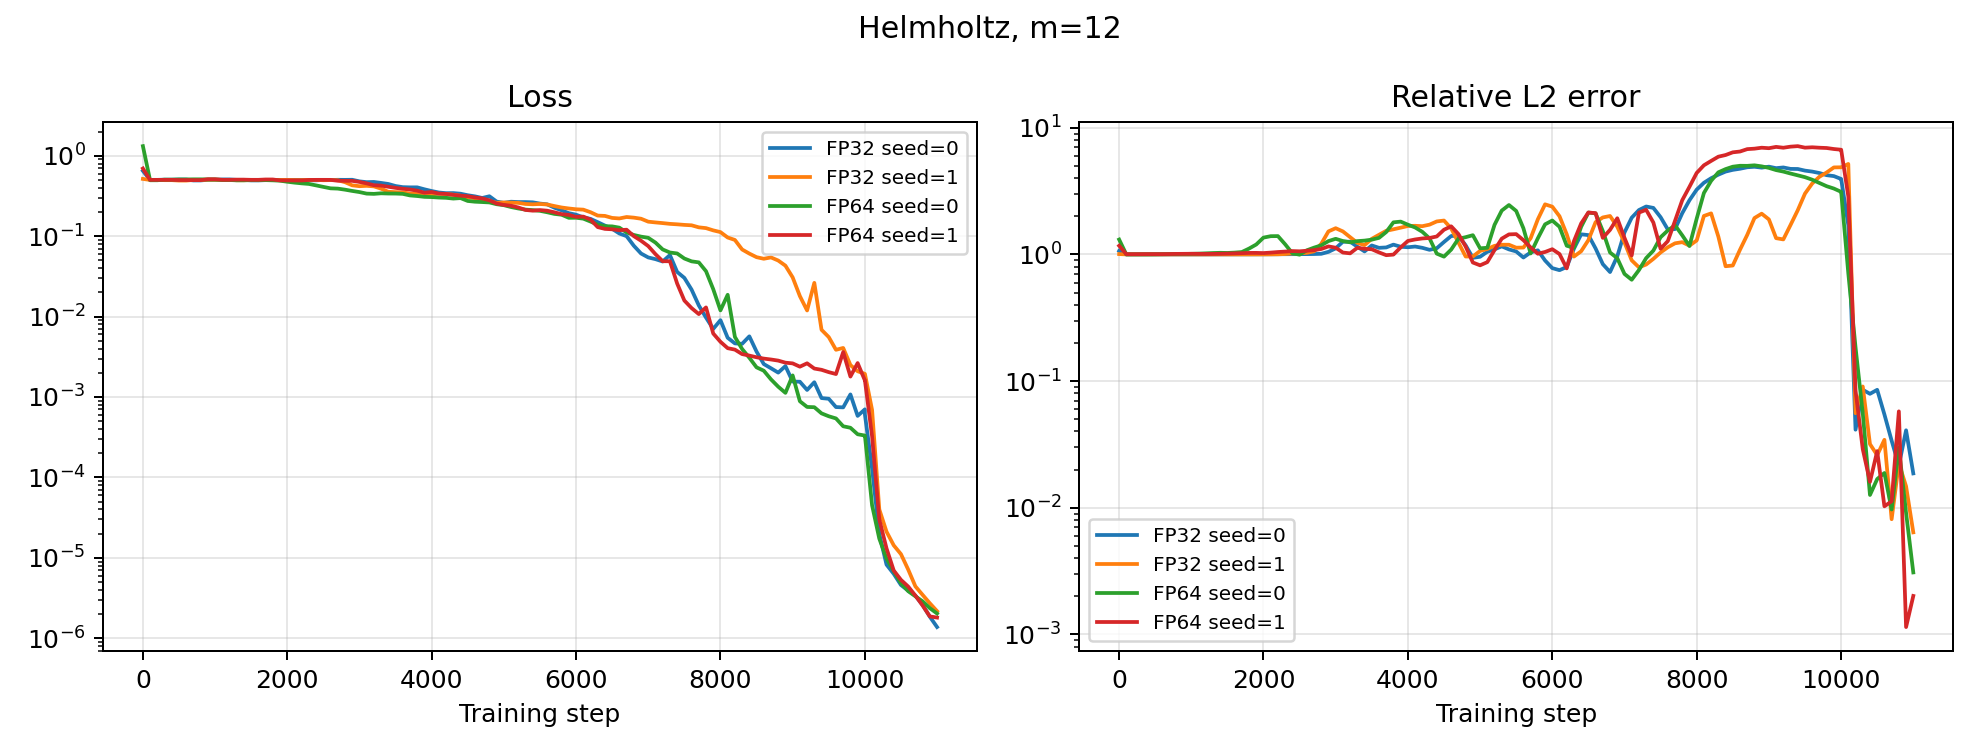
\includegraphics[width=0.9\textwidth]{report_results/figures/report_helmholtz_m12_curves.png}
    \caption{Кривые обучения для Helmholtz1D, $m=12$}
    \label{fig:helmholtz_m12_curves}
\end{figure}

\begin{figure}[H]
    \centering
    \begin{subfigure}{0.48\textwidth}
        \centering
        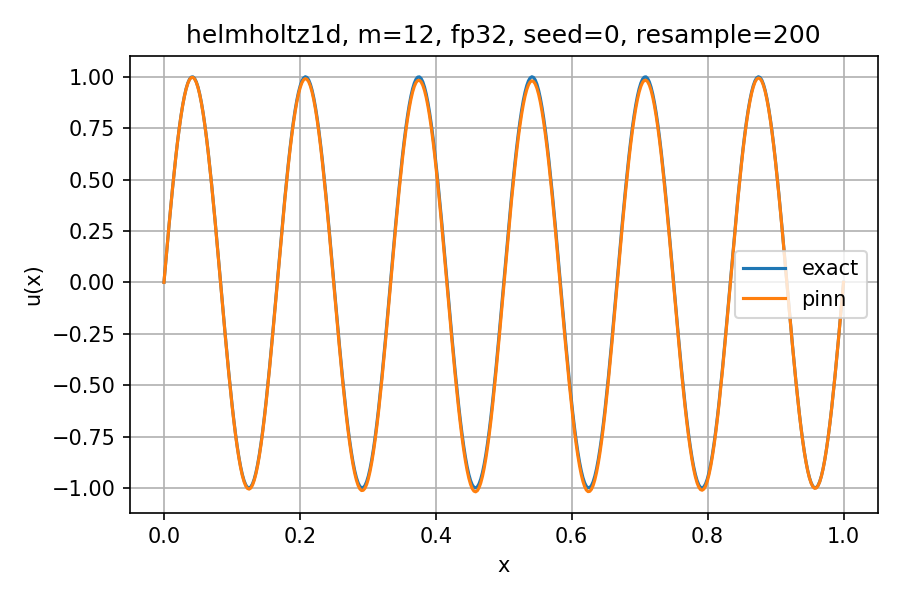
\includegraphics[width=\textwidth]{report_results/figures/solution_slices/helmholtz_m12_fp32_seed0.png}
        \caption{FP32}
    \end{subfigure}
    \hfill
    \begin{subfigure}{0.48\textwidth}
        \centering
        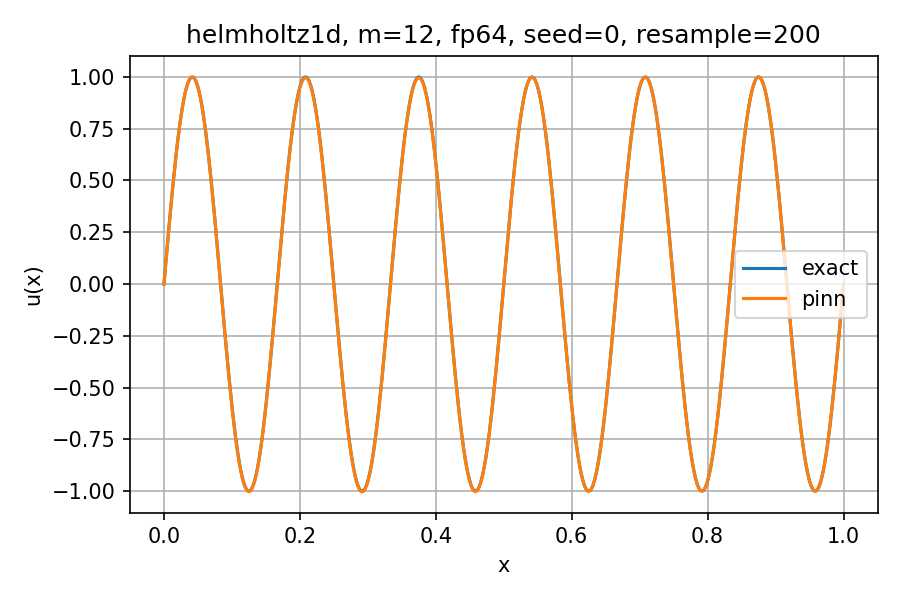
\includegraphics[width=\textwidth]{report_results/figures/solution_slices/helmholtz_m12_fp64_seed0.png}
        \caption{FP64}
    \end{subfigure}
    \caption{Фактические решения для Helmholtz1D, $m=12$}
    \label{fig:helmholtz_m12_solution_slices}
\end{figure}


Кривые на рисунке~\ref{fig:helmholtz_m12_curves} показывают, что различие между FP32 и FP64 связано не только с финальным числом в таблице. В FP64 обучение продолжает улучшать решение до меньшей ошибки, тогда как FP32 в некоторых запусках останавливается на более высоком уровне ошибки. Это согласуется с гипотезой о том, что численная точность может влиять на прохождение failure modes в PINN.

\subsection{Convection1D}

Задача Convection1D используется как дополнительный baseline, близкий к failure-mode постановкам из литературы. В основной части работы рассматривается случай $\beta=30$. Более сложный случай $\beta=50$ не используется как главный результат, потому что он сильнее зависит от seed и требует большего числа запусков для аккуратного вывода.

Для $\beta=30$ были получены следующие результаты.

\begin{table}[H]
\centering
\caption{Результаты на Convection1D}
\label{tab:convection_results}
\begin{tabular}{lllll}
\hline
Задача & Параметр & Seed FP32/FP64 & FP32 best L2 & FP64 best L2 \\
\hline
Convection1D & $\beta=30$ & 2/2 & \num{1.094e-2} & \num{6.625e-3} \\
\hline
\end{tabular}
\end{table}

В таблице~\ref{tab:convection_results} видно умеренное улучшение при переходе к FP64. Отношение FP64/FP32 для этого случая равно примерно $\num{0.606}$. Это означает, что FP64 даёт меньшую ошибку, но эффект не такой сильный, как в основных Helmholtz-запусках.

\begin{figure}[H]
    \centering
    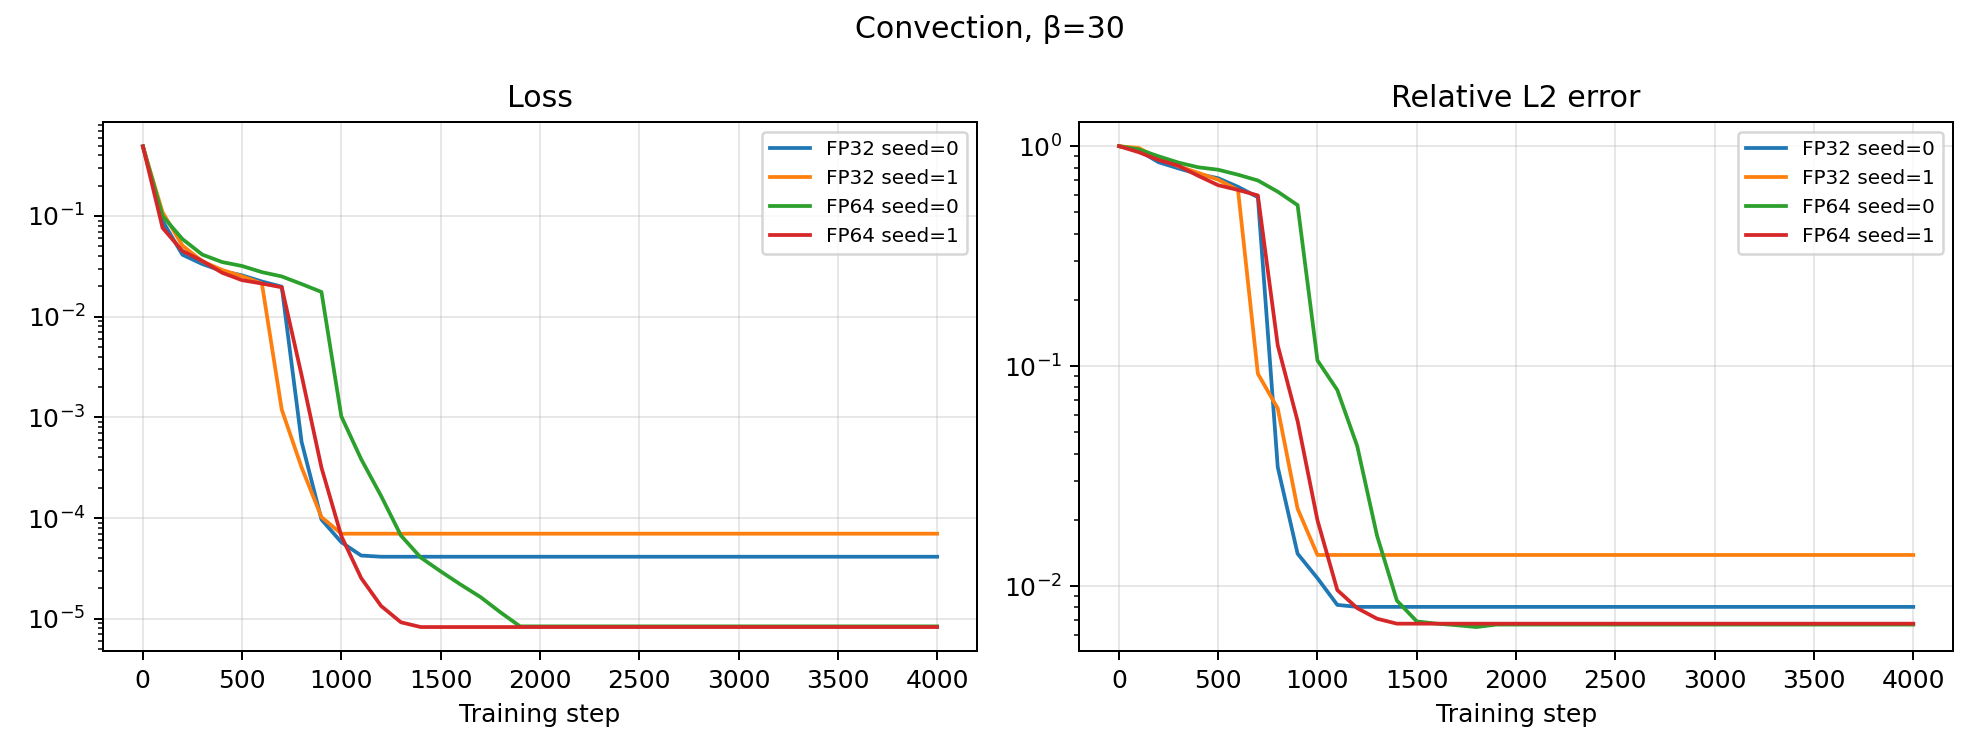
\includegraphics[width=0.9\textwidth]{report_results/figures/report_convection_beta30_curves.png}
    \caption{Кривые обучения для Convection1D, $\beta=30$}
    \label{fig:convection_beta30_curves}
\end{figure}

\begin{figure}[H]
    \centering
    \begin{subfigure}{0.48\textwidth}
        \centering
        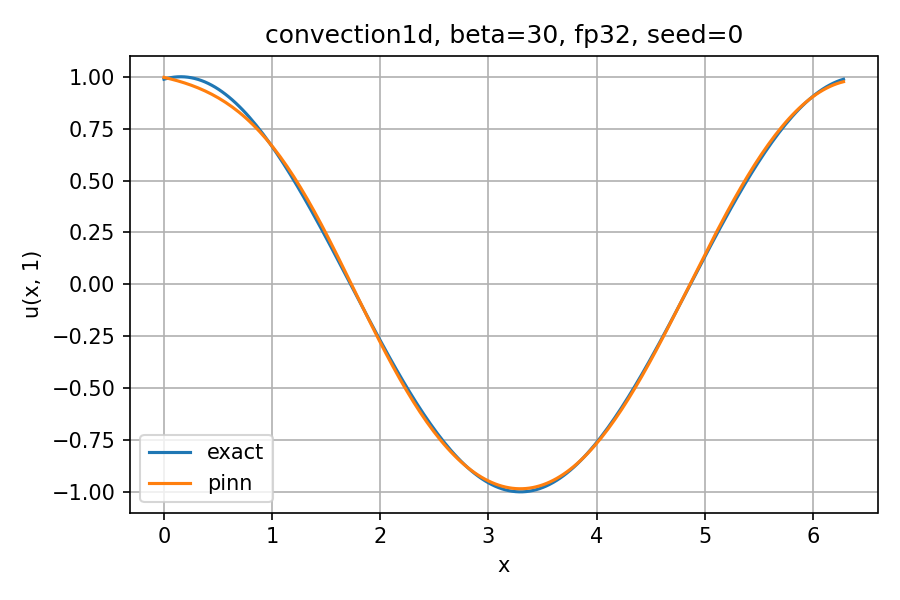
\includegraphics[width=\textwidth]{report_results/figures/solution_slices/convection_beta30_fp32_seed0.png}
        \caption{FP32}
    \end{subfigure}
    \hfill
    \begin{subfigure}{0.48\textwidth}
        \centering
        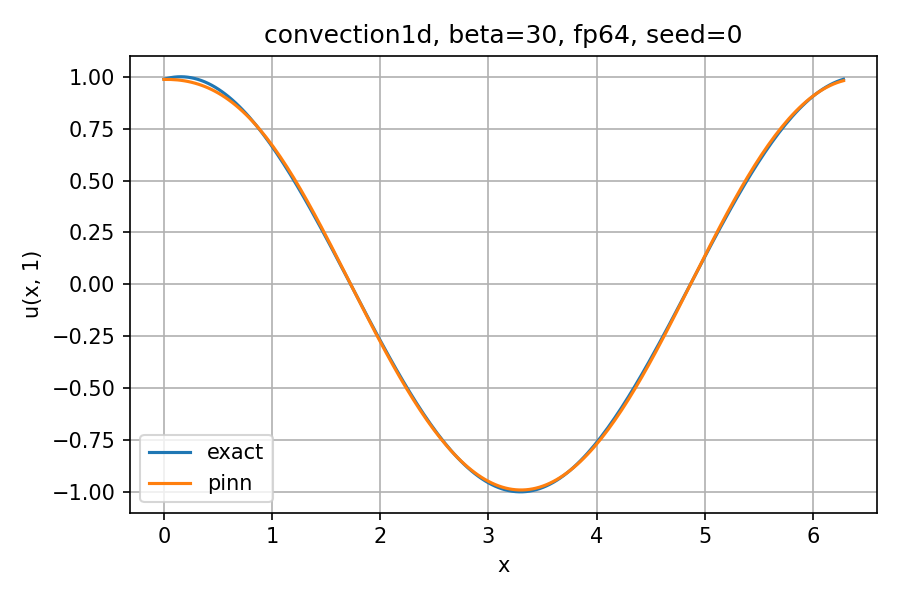
\includegraphics[width=\textwidth]{report_results/figures/solution_slices/convection_beta30_fp64_seed0.png}
        \caption{FP64}
    \end{subfigure}
    \caption{Фактические решения для Convection1D, $\beta=30$}
    \label{fig:convection_beta30_solution_slices}
\end{figure}


Кривые обучения на рисунке~\ref{fig:convection_beta30_curves} показывают, что Convection1D остаётся чувствительной задачей для PINN. При этом в данном эксперименте FP64 даёт более низкую медианную ошибку, но этот результат используется как дополнительная проверка, а не как главный вывод работы.

\subsection{Burgers1D: смешанный пример}

Задача Burgers1D нужна для проверки того, является ли преимущество FP64 универсальным. В отличие от Helmholtz1D, здесь результаты оказались смешанными.

\begin{table}[H]
\centering
\caption{Результаты на Burgers1D}
\label{tab:burgers_results}
\begin{tabular}{lllll}
\hline
Задача & Параметр & Seed FP32/FP64 & FP32 best L2 & FP64 best L2 \\
\hline
Burgers1D & $\nu=0.002$ & 2/2 & \num{4.878e-2} & \num{4.652e-2} \\
Burgers1D & $\nu=0.001$ & 2/2 & \num{9.485e-2} & \num{1.700e-1} \\
\hline
\end{tabular}
\end{table}

При $\nu=0.002$ FP32 и FP64 дают близкие результаты: медианная лучшая относительная L2-ошибка равна $\num{4.878e-2}$ для FP32 и $\num{4.652e-2}$ для FP64. Разница есть, но она небольшая.

При $\nu=0.001$ ситуация меняется. FP64 даёт худшую медианную ошибку, чем FP32. Для FP32 ошибка равна $\num{9.485e-2}$, а для FP64 - $\num{1.700e-1}$.

\begin{figure}[H]
    \centering
    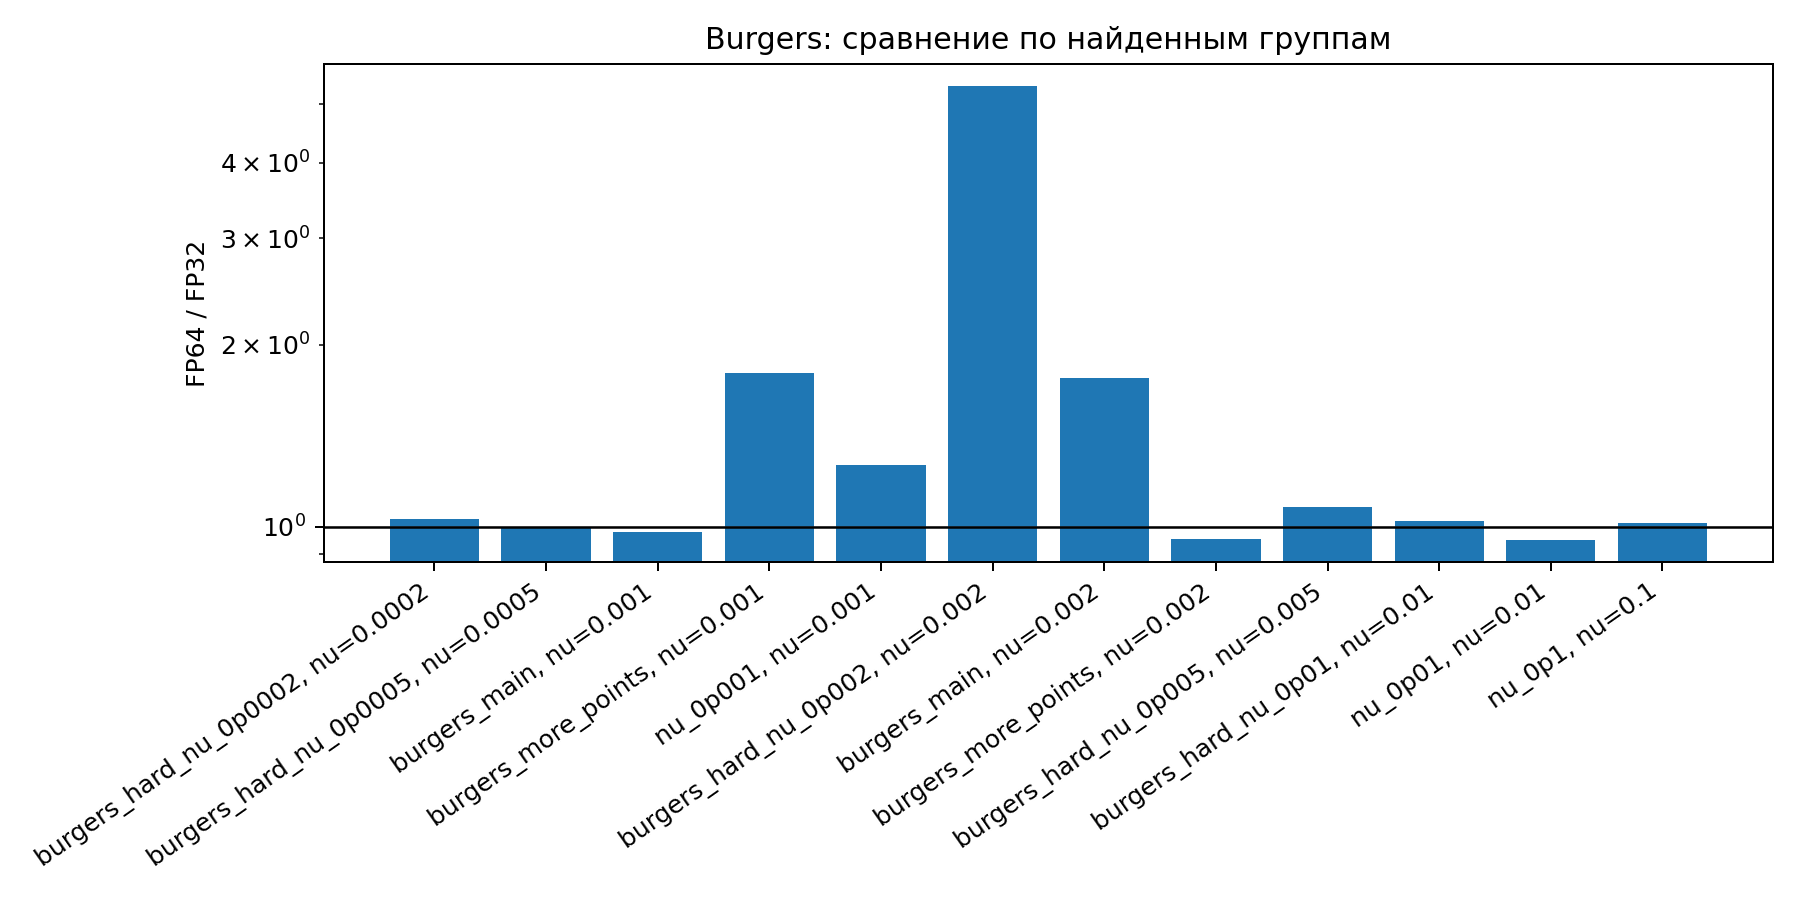
\includegraphics[width=0.85\textwidth]{report_results/figures/report_burgers_summary.png}
    \caption{Сравнение FP32 и FP64 на Burgers1D}
    \label{fig:burgers_summary}
\end{figure}

\begin{figure}[H]
    \centering
    \begin{subfigure}{0.48\textwidth}
        \centering
        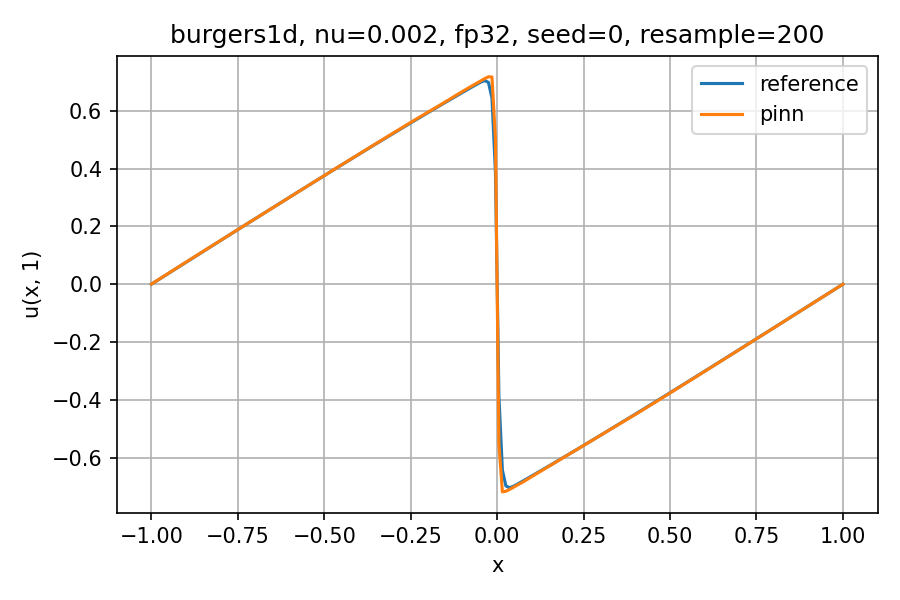
\includegraphics[width=\textwidth]{report_results/figures/solution_slices/burgers_nu0p002_fp32_seed0.png}
        \caption{FP32}
    \end{subfigure}
    \hfill
    \begin{subfigure}{0.48\textwidth}
        \centering
        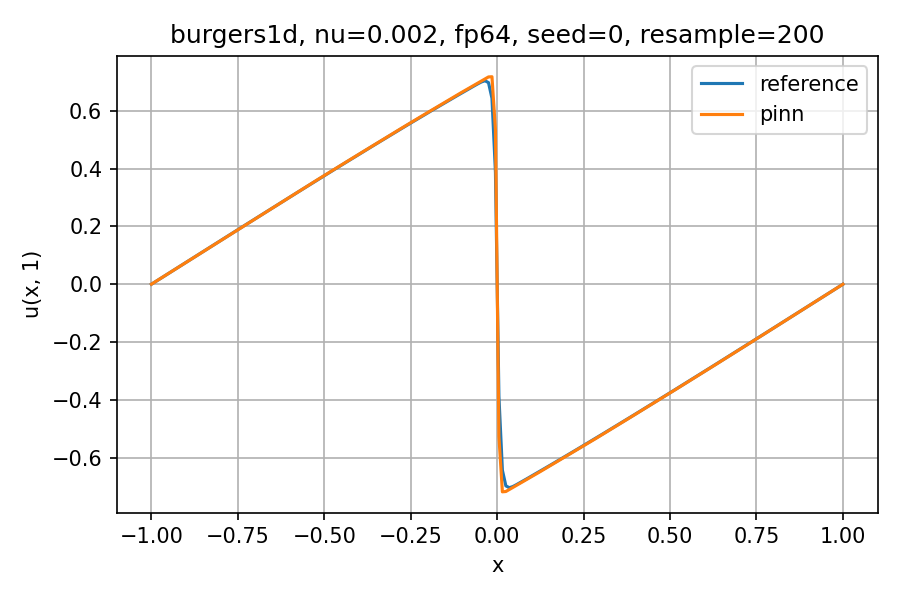
\includegraphics[width=\textwidth]{report_results/figures/solution_slices/burgers_nu0p002_fp64_seed0.png}
        \caption{FP64}
    \end{subfigure}
    \caption{Фактические решения для Burgers1D, $\nu=0.002$}
    \label{fig:burgers_nu0p002_solution_slices}
\end{figure}


Рисунок~\ref{fig:burgers_summary} подтверждает смешанный характер результатов на Burgers1D. В этой задаче на качество обучения влияют не только ошибки округления, но и сложность самой PDE, архитектура модели и работа оптимизатора.


\section{Обсуждение результатов}

Главный положительный результат получен на Helmholtz1D. В нескольких запусках FP64 даёт меньшую относительную L2-ошибку, чем FP32. Особенно заметен случай $m=12$, где ошибка уменьшается с $\num{1.253e-2}$ до $\num{2.114e-3}$ в одном из основных режимов. Это хорошо согласуется с идеей, что в некоторых PINN-задачах численная точность влияет не только на финальное значение метрики, но и на сам ход оптимизации.

Задача Heat1D успешно решается при любой точности поэтому использование ресурсоемкого FP64 здесь нецелесообразно.

Convection1D при $\beta=30$ даёт умеренное улучшение при переходе к FP64.

Burgers1D не подтверждает гипотезу. При $\nu=0.002$ результаты FP32 и FP64 близки, а при $\nu=0.001$ FP64 оказался хуже. Значит, повышенная точность сама по себе не решает все проблемы обучения PINN. Скорее всего проблема failure mode здесь вовсе не возникла и функция потерь не достигла достаточно малых значений для этого. Для реальной проверки гипотезы необходимы более устойчивые запуски.

Важным фактором определяющим режим failure mode при использовании FP32 в PINN является ограничение $\epsilon\approx1.19*10^{-7}$. В L-BFGS стандартно критерий остановки задается равным $\approx 10^{-7}$. Таким образом при приближении значения функции потерь к порядку $\approx10^{-7}$, появляется нустранимая погрешность измерения и L-BFGS воспрнимает полученный шум как отсутствие значимого убывания лосса и останавливает обучение. Переход к FP64 сильно сдвигает данный барьер поскольку уменьшается до $\epsilon \approx 2.22 * 10^{-16}$ Это позволяет L-BFGS продолжать корректное вычисление производных высших порядков и шагов оптимизации в сложных задачах.


\section{Заключение}

Работа подтверждает, что значительная часть известных режимов сбоя при обучении PINN носит не структурный характер, а чисто оптимизационный. Необходимость использования высокой точности напрямую зависит от характера ландшафта потерь конкретной физической задачи:

Для гладких диффузионных процессов (Heat1D) точности FP32 достаточно для достижения высокого качества, и избыточные вычисления нецелесообразны.

Для жестких задач с высокой частотой колебаний (Helmholtz1D) высокая разрядность критически необходима для преодоления оптимизационных барьеров.

Для задач с сильной нелинейностью (Burgers1D) переход на FP64 сам по себе не решает проблему застревания в плохих локальных минимумах, что указывает на необходимость комбинации высокой точности со специальными методами сэмплирования или изменения архитектуры.


\clearpage

\phantomsection
\addcontentsline{toc}{section}{Список литературы}
\bibliography{bib}


\clearpage

\appendix
\section*{Приложение}
\addcontentsline{toc}{section}{Приложение}

\subsection*{Пробные запуски FP16}
\addcontentsline{toc}{subsection}{Пробные запуски FP16}

\begin{figure}[H]
    \centering
    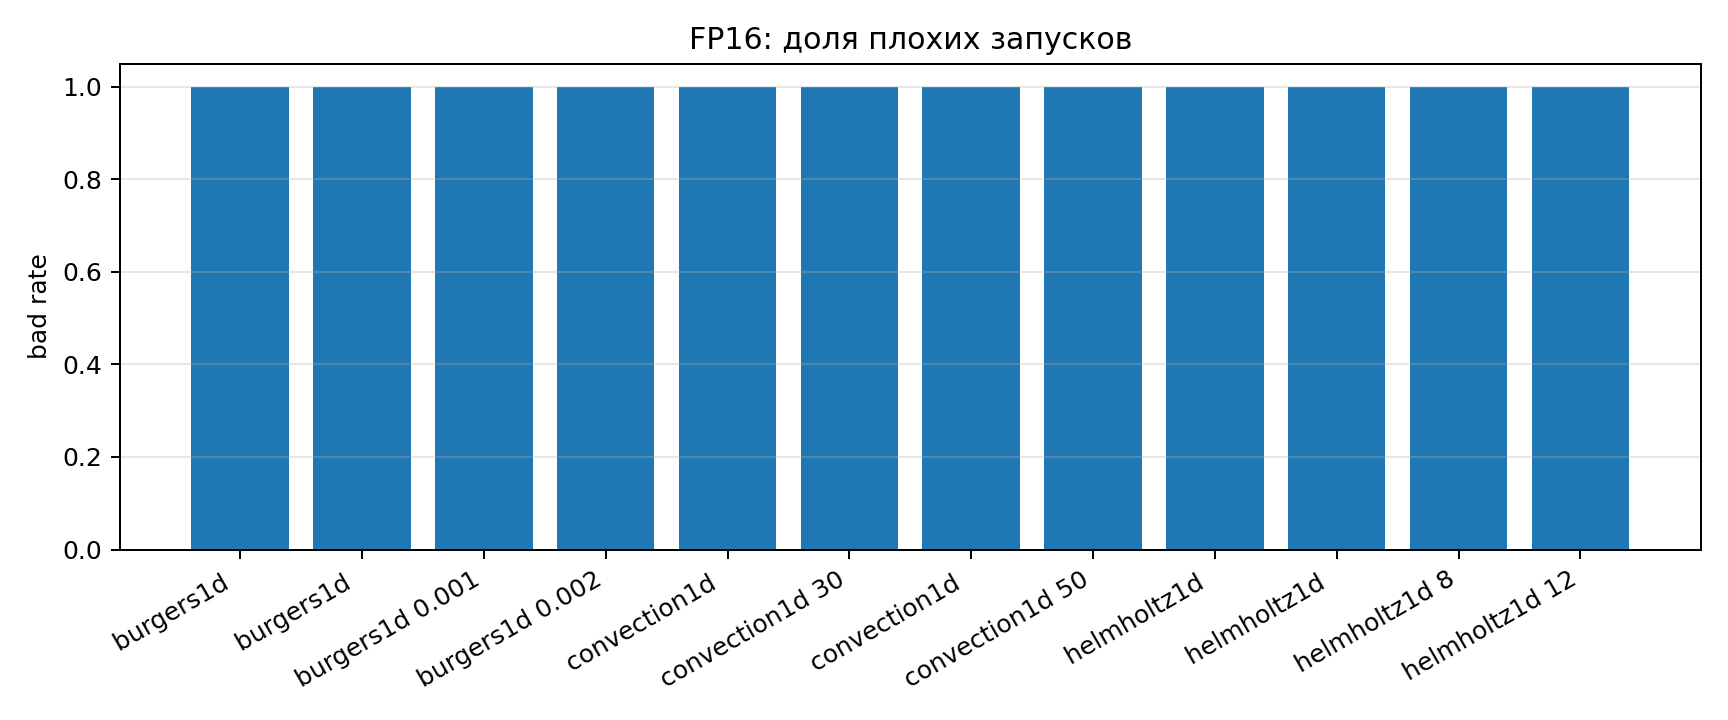
\includegraphics[width=0.9\textwidth]{report_results/figures/report_fp16_summary.png}
    \caption{Сводка пробных запусков FP16}
    \label{fig:fp16_summary_appendix}
\end{figure}

В рамках работы были проведены тестовые запуски обучения PINN в формате FP16. Данный формат не был включен в основную экспериментальную часть исследования, поскольку во всех тестах он показал критическую нестабильность оптимизации.
В PINN функция потерь вычисляется через автоматическое дифференцирование и невязку PDE. Значения градиентов высших порядков часто оказываются меньше, чем минимально представимое число в FP16 ($6.10*10^{-5}$), что приводит к их занулению. Так же дискретность сетки FP16 порождает сильный численный шум, из-за чего оптимизатор L-BFGS прерывает работу.

\end{document}

